\documentclass[11pt,a4paper,oneside]{book}
\usepackage[hmargin={1.25in,1.25in},vmargin={1.25in,1.25in}]{geometry}

\makeindex
\usepackage{textcomp}
\usepackage{fancyhdr}
\usepackage{makeidx}
\pagestyle{myheadings}
\fancyhf{}
\rhead[\leftmark]{thepage}

\usepackage[latin1]{inputenc}
\usepackage{url}


% for argmin formula operator
\usepackage{amsmath}
\DeclareMathOperator*{\argmax}{arg\,max}
\DeclareMathOperator*{\argmin}{arg\,min}

% for listings
\usepackage{listings}
\lstset{
numbers=left, 
numberstyle=\small, 
numbersep=8pt, 
frame = single, 
breaklines=true,
tabsize=2,
framexleftmargin=15pt}

% for images
\usepackage{graphicx}
\graphicspath{{./images/}}

% enables click hyperreferences
\usepackage{hyperref}

% for multiple images on a row
\usepackage{multicol}
\usepackage{lipsum}
\usepackage{mwe}

% for several pages table
\usepackage{longtable}

\parindent0em
\parskip1.5ex

\begin{document}

\frontmatter
\begin{titlepage}
\begin{center}
\textbf{UNIVERSIT\'E LIBRE DE BRUXELLES}\\
\textbf{Facult\'e des Sciences}\\
\textbf{D\'epartement d'Informatique}
\vfill{}\vfill{}

{\Huge Development of an automatically configurable ant colony optimization framework for vehicle routing variants}

{\Huge \par}
\begin{center}{\LARGE Aldar Saranov}\end{center}{\Huge \par}
\vfill{}\vfill{}
\begin{flushright}{\large \textbf{Promoter :} Prof. Thomas St{\"u}tzle}\hfill{}{\large Master Thesis in Computer Sciences}\\
{\large }\hfill{}{}\end{flushright}{\large\par}
\vfill{}\vfill{}\enlargethispage{3cm}
\textbf{Academic year 2016~-~2017+1}
\end{center}
\end{titlepage}
\newpage
\thispagestyle{empty} 
\null

\newenvironment{vcenterpage}
{\newpage\thispagestyle{empty} 
\vspace*{\fill}}
{\vspace*{\fill}\par\pagebreak}

\begin{vcenterpage}
\begin{flushright}
    \large\em\null\vskip1in 
    Dedicated to my mother Lena, who\\
   was always sincerely supporting me\vfill
  \end{flushright}
\end{vcenterpage}
\thispagestyle{empty}
\vspace*{5cm}

\begin{quotation}
\noindent ``\emph{If one does not know to which port one is sailing, no wind is favorable.}''
\begin{flushright}\textbf{Lucius Annaeus Seneca, 1st century AD}\end{flushright}
\end{quotation}

\medskip

\begin{quotation}
\noindent ``\emph{The general, unable to control his irritation, will launch his men
to the assault like swarming ants, with the result that one-third of
his men are slain, while the town still remains untaken. Such are
the disastrous effects of a siege.}''
\begin{flushright}\textbf{Sun Tzu, "The Art of War", 5th century BC}\end{flushright}
\end{quotation}
\chapter*{Acknowledgment}
\thispagestyle{empty} 

\noindent I want to thank my promoter, prof. Thomas St{\"u}tzle, whose determination and competencies were leading me to the goal of the paper, and my friend, Alain, who made this precious time of my education possible.

\thispagestyle{empty} 
\setcounter{page}{0}
\tableofcontents
\mainmatter 
\chapter{Introduction}
\setcounter{page}{1}
\vspace*{0.5cm}

Some insect species show an extreme degree of social organization. For example many ant species have pheromone production and detection body parts and therefore seize an ability to communicate between each other in an indirect way. Such indirect communication between organism is called stigmergy. Biologists conducted several experiments with ant colonies initiating their foraging behavior and found out that they tend to find shortest paths between the nest and food sources by means of such communication. This concept has inspired the development of algorithms, which are based on the social behavior of ant colonies, called ant colony optimization (ACO) algorithms. ACO algorithms solve NP-hard problems in a very efficient manner \cite{Dorigo1996}. These algorithms are considered to be metaheuristics. By metaheuristic we imply a generic set of rules for deriving heuristic algorithms. As for the ACO metaheuristic, it includes also the possibility of local search: once ants complete their solution construction phase, local search algorithms can be used to refine their solutions before using them for the pheromone update. Various experimental researches have shown that the combination of solution cconstruction by ants and local search procedures is a promising approach. ACO algorithms have a large number of variations and configuration parameters, that drastically influence the algorithm performance. These parameters may be unified by means of some framework.

At the moment, there exists a state-of-the-art software called ACOTSPQAP. As the name says, it is designed to solve the Traveling Salesman Problem and the Quadratic Assignment Problem with high-efficiency by means of ACO meta-heuristics. It also includes different algorithm variations as Ant System (AS), Elitist Ant System (EAS) \cite{Dor1992:thesis,Dorigo1996}, Max-Min Ant System (MMAS) \cite{STUTZLE2000889}, Rank-based Ant System (RAS) \cite{Bullnheimer97anew}, Best-Worst Ant System (BWAS) \cite{Cordon00anew}, Ant Colony System (ACS) \cite{Dorigo1997}. As for the implementation, it is written in C and, therefore, it adheres to the structural programming paradigm. Although adapting the software to a different problem type context is possible, it is nonetheless more costly than if it was written according to the object-oriented programming (OOP) paradigm. OOP reduces cost, due to its essential properties (inheritance, abstraction and polymorphism). These properties may heavily reduce code repetition. For example having implemented an abstraction of an NP-hard problem and one of its implementations for one concrete NP-hard problem, one will only have to make another implementation of the problem abstraction for the respective problem type, in case if switching to another problem type is required. These implementations contain only problem specific parts of the code and are mutually replaceable. In structured programming however, the program is split into high and low level modules, and in case of program extension both high and low level modules will be subject to modification.

The development of a flexible OOP driven ACO framework is the next step of formalizing this area. Such a framework can then be used as a tool to help solving various optimization problems. This thesis gives a brief overview of the current state of the ACO research area, existing framework description and some tools which can be used for the automatic configuration of the framework.

The work was started by analyzing and aggregating possible options and choices, trying to define their common parts in order to derive abstract classes and reduce component repetitions. In chapter 2, we describe the theoretical foundation of the framework, that is required to be developed. However, unreasonable selection of an ACO algorithm configuration may lead to low-quality results even after a long execution. A simple decision is to perform a configuration tuning before the actual execution. This chapter also introduces a description of a configuration software called irace, that allows to obtain high-performing configurations for further framework exploiting. We adapted the developed framework for use with irace by giving a specification of the framework parameter space.

The development of such framework would also require its application to some particular problem for testing and analysis purposes. Vehicle Routing Problem (VRP) was chosen as the one. It is a widely researched NP-hard combinatorial optimization problem, therefore, it will allow us to perform a benchmark comparison with publicly available problem instances, that we obtain. In chapter 3, we introduce formulation of VRP and also mention several variations thereof.

In chapter 4, we describe the implementation details and decisions for the ACO framework, the way we adapt it specifically to VRP-problems and we also show a line-by-line description of the parameter space defined for the framework. We also explain there how we attain high flexibility of the framework in order to adapt it for various problem types besides VRP.

In chapter 5, one can see the experimental set-up, tuning results, performance benchmark and verbal interpretations of the results.

In chapter 6, we finalize the work, list conclusion remarks and give a short overview of results of each step. In addition, we emphasize the application areas, where this framework may be useful. 

\chapter{Background}

\section{Combinatorial Optimization Problems and Constructive Heuristics}

Combinatorial optimization problems (COPs) are a large class of mathematical optimization problems. These problems can be described as a grouping, ordering, assignment or any other operations over a set of discrete objects. In practice, one may need to resolve COPs, which have a large number of extra constraints for the solutions to consider them as admissible. Many of these problems which are still being thoroughly researched at the moment, belong to NP-hard discrete optimization problems. The best performing algorithms known today to solve such problems have a worst-case run-time larger than polynomial (e.g. exponential).

\noindent\fbox{%
    \parbox{\textwidth}{%
\underline{An Optimization Problem} is a tuple \cite{papadimitriou1982combinatorial} ($\Phi,\omega, f$), where
	\begin{itemize}
		\item{$\Phi$ is a \underline{search space} consisting of all possible assignments of discrete variables $x_i$, with $i=1,...,n$ }
		\item{$\omega$ is a \underline{set of constraints} on the decision variables}
		\item{$f:\Phi \to R$ is an \underline{objective function}, which has to be optimized}
	\end{itemize}
    }%
}

The problem formulation describes an abstract task (e.g. find the minimum spanning tree of some graph), while the instance of a problem describes a specific practical problem (e.g. find the minimum spanning tree of a given graph G). The objective function is the sum of the weights of the selected edges. \par

Any combination of solution components is called a candidate solution (not necessarily satisfying all problem constraints). Oppositely, solution is a candidate solution, that satisfies all problem constraints.

Since solving of NP-hard problems by trying to find provably optimal solutions is unreasonable, one can apply heuristic algorithms, which more or less provide solutions with relatively good quality consuming reasonable quantity of resources (time/power, memory etc.). An important class of such heuristic algorithms are constructive heuristics. Constructive heuristics start with an empty or partially built solution, which is then being completed by iterative extension until a full solution is completed. Each of the iterations adds one or several solution components to the solution. For example, greedy constructive heuristics  add the best-ranked components by their heuristic values.




\section{Ant Colony Optimization}

ACO algorithms are a subclass of constructive heuristics. Meta-heuristic is a top-level heuristic, which is used to improve the performance of an underlying, basic heuristic. ACO is such a metaheuristic that can be used to improve the performance of a construction heuristic. One has to remark several necessary features of the ACO algorithms:

\begin{itemize}
\item ACO algorithms are population-based algorithms. Solutions are being generated at each iteration.
\item Solutions are being generated according to a probability-based mechanism, which is biased by artificial pheromones that are assigned to problem specific solution components.
\item The quality of the generated solutions affect the pheromones, which are updated during the run of the algorithm.
\end{itemize}


\begin{minipage}[c]{0.95\textwidth}
\begin{lstlisting}[caption={General ACO pseudo-code}, label={lst:aco}]
procedure ACO-Metaheuristic
repeat
	foreach ant do
		repeat
			extend-partial-solution-probabilistically()
		until solution-is-complete()
	
	foreach ant in select-ants-for-local-search() do
		apply-local-search(ant)
	
	evaporate-pheromones()
	deposit-pheromones()
until termination-criteria-met()
end
\end{lstlisting}
\end{minipage}

Pheromones are numeric values associated to the solution components that are meant to bias the solution construction in order to improve the quality of the generated solutions. Several ants generate the solutions by an iterative approach (see Listing \ref{lst:aco}). After this, an optional local search is applied. Next, pheromone evaporation and deposit is done. Evaporation helps to reduce the convergence-prone behavior of the algorithm. Deposit is the part where the solutions affect the pheromone values in order to bias the future solutions.

\subsection{Choice of pheromone trails and heuristic information}

Generally, there are two mechanisms of biasing the solution construction - pheromones and heuristic values. \\
Hereby we introduce the following components: \\
$C$ - set of solution components (a combination of which can constitute a solution). \\
$\tau_c \in T$ - pheromones trail values for solution component bias. \\
$\tau'_c \in T'$ - pheromones trail values for particular purposes. \\
$\pi$ - candidate solution. \\
$\eta_c \in H$ - heuristic information (constant in time). \\

Higher values of $\tau_c$ stand for a higher probability that the component $c$ will be added to a solution. Additionally, problem-specific pheromones such as $\tau'_c$ can be used for auxiliary purposes. 

Similarly heuristic values are numerical attributes of the solution components. However, generally heuristic values are assigned as constants at the start of the solution construction, although in extensions one can use heuristic values, which are a function of the generated partial solution. These are called \emph{adaptive} heuristics and normally they consume larger computer resources although they often lead to a better quality of the generated solutions. Heuristic information $H$ is similar to the pheromone trails in terms of that they both bias the solution component choice. However, it is defined in problem-specific way and is not updated during the algorithm execution ($\forall c \in C, \exists \eta_c \in H$). Heuristic information is either static values or values which are defined by a function of the current partially constructed solution. 

\subsection{Solution component choice}

The solution construction phase, as says the name, yields a new solution set. The probability of $c_j$ to be added at a certain step can be calculated by different techniques (i.e. $Pr(c_j|T,H,s)$). Each ant starts with an empty solution $s$. Each ant may produce one solution at one execution of the solution construction phase. At each construction step one solution component is added. A frequently used rule is defined as follows:

\begin{equation}
Pr(c_j)=\frac{t_j^\alpha \times \eta_j^\beta}{\sum \limits_{c_k \in N_i} t_k^\alpha \times \eta_k^\beta} \forall c_j \in N_i
\label{eq:construction_classic}
\end{equation}

$\alpha$ and $\beta$ are parameters that determine the impact of the pheromone trails and heuristic information on the final probability. Another alternative has been proposed by Maniezzo \cite{Maniezzo1999}, which combines the pheromone trails and heuristic information in a linear way.

\begin{equation}
Pr(c_j)=\frac{\alpha \times \tau_j + (1-\alpha) \times \eta_j}{\sum \limits_{c_k \in N_i} \alpha \times \tau_k + (1-\alpha) \times \tau_k} \forall c_j \in N_i
\label{eq:construction_maniezzo}
\end{equation}

Since it does not use exponentiation operations such choice rule is preferable for performance-targeted frameworks. However, this algorithm may cause undesired biases if the range of the values are not taken into account. The third alternative is invented by Dorigo and Gambardella \cite{Dorigo1997} in Ant Colony System (ACS) algorithm. The rule of solution component choice in ACS is also called pseudo-random proportional rule. A random uniform value $q$ is generated in range $[0;1)$ and if $q>q_0$, where $q_0$ is a predefined parameter, then the probability of choosing $c_j$ is calculated according to formula \eqref{eq:construction_classic}. Otherwise, the solution component is picked as:

\begin{equation}
c_j = \operatornamewithlimits{argmax}\limits_{c_k \in N_i} t_k^\alpha \times \eta_k^\beta
\label{eq:construction_dorigo}
\end{equation}

Apparently, larger $q_0$ gives more greedy choice.

\subsection{Construction extensions}

\textbf{Lookahead} concept was introduced. It says that at each decision step several solution components should be considered at once in order to get the next solution component \cite{10.1007/BFb0056911}. This says that in constructing a candidate solution, ants use a transition rule that incorporates complete information on past decisions (\emph{the trail}) and local information (\emph{visibility}) on the immediate decision that is to be made. The look-ahead mechanism allows the incorporation of information of the anticipated decisions that are beyond the immediate choice horizon. Generally, it is worth to be implemented when the cost of making a local prediction based on the current partial solution state is much lower than the cost of the real execution of the move sequence.

\textbf{A candidate list} restricts the solution component set to a smaller set to be considered. The solution components in this list have to be the most promising ones at the current step \cite{782657,Dorigo1997}. Usually, this approach yields a significant gain of computation time, depending on the initial set-up (i.e. if this list is precalculated once before the run). Nonetheless, it can also depend on the current partial solution.


\textbf{Hash table} of pheromone trails. It allows to efficiently save memory when the updated pheromone trails are in a sparse set in comparison to the set of all solution components. Search and updating of the elements of the hash-table is expected to be done within linear time \cite{DBLP:conf/gecco/AlbaC07}.

\textbf{Heuristic precomputation} of the values $t_j^\alpha \times \eta_j^\beta$ for each of the solution components which are used in formula \eqref{eq:construction_dorigo}. The reduction of computation time is based on the fact that all these values will be shared by the ants at each iteration.

\textbf{External memory} extension is based on starting the solution construction from a partially constructed solution with partial destroying of a certain good solution and reconstructing it and thus anticipating to obtain even a better solution. This iterated greedy extension was inspired by genetic algorithms and described in \cite{10.1007/978-3-540-28646-2_7}. It uses reinforcement procedures of the elite solutions with deferred reintroducing of solutions segments in following iterations, see Listing \ref{lst:ext-mem}. The ACO iteration is composed of two stages. First is meant to initialize the external memory. The second is the solution construction itself based on a partial solution. 

\begin{minipage}[c, breaklines=true]{0.95\textwidth}
\begin{lstlisting}[caption={External memory iteration pseudo-code}, label={lst:ext-mem}]
procedure ACO-external-memory
initialize the external memory
repeat
	set m ants in the graph
	
	ants construct a solution using neighborhood graph and the pheromone matrix
	
	select k-best solutions and cut randomly positioned and sized segments
	
	store the segments into the external memory
until the external memory is full

done = false

while not(done)
	ants select their segments according to tournament selection
	
	ants finish the solution construction
	update the pheromone matrix
	update the memory
end
end
\end{lstlisting}
\end{minipage}

Tournament selection procedure is usually defined as follows: from a set of solutions, one selects randomly $tSize$ solutions, finds the best solution among them and places this solution into result set. This is repeated $m$ times.

\textbf{Iterated ants} also uses the partially constructed solutions. Based on the following additional notions. Destruct() removes some solution components from a complete solution \cite{10.1007/11839088_16}. Constuct() constructs a complete solution from initially partial solution. An acceptance-criterion chooses one of two complete solutions in order to continue the construction with it. Concrete implementations of these strategies are defined in problem-specific way. The algorithm of the extension is showed in Listing \ref{lst:iterated-ants}.

\begin{minipage}[c, breaklines=true]{0.95\textwidth}
\begin{lstlisting}[caption={General iterated ants pseudo-code}, label={lst:iterated-ants}]
procedure iterated-ants
	s0 = initial-solution()
	s = local-search(s0)
	repeat
		sp = destruct(s)
		s' = construct(sp)
		s' = local-search(s')   // optional
		s = acceptances-criterion(s,s')
	until termination criterion met
end
\end{lstlisting}
\end{minipage}

\textbf{Cunning ants} algorithm tackles to the solution generation by iterated producing of new ant population. The algorithm has a pheromone database and an ant population of fixed size. For every existing ant, a new one is produced which borrows some solution parts from its parent \cite{Tsutsui2007}. Then in each such ant pair a winner is selected and all winners continue their work in the next iteration. After each iteration all winners jointly update the pheromone database and stop if the termination criteria is met. Similarly the solution component inheritance process is problem-specific.

As an extension of the original cunning ants variation, one may use local search after the reconstruction step and also a custom pheromone update algorithm. The cunning ants algorithm is illustrated on Figure \ref{fig:cunning-ants}.

\begin{figure}[h]
  \centering
    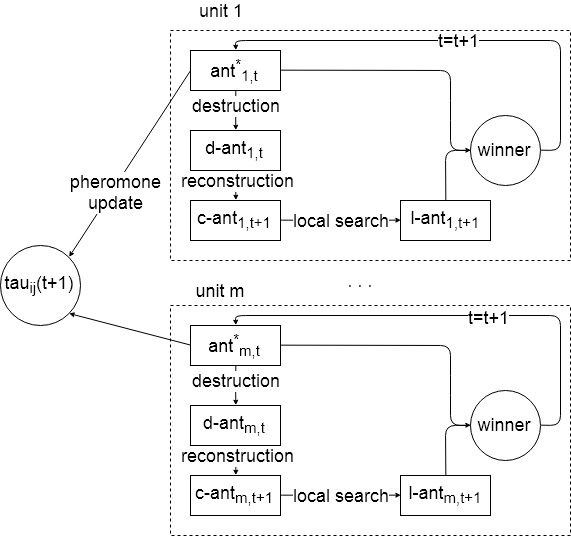
\includegraphics[scale=0.5]{cunning-ants.jpg}
  \caption{Cunning ants}
  \label{fig:cunning-ants}
\end{figure}


\subsection{Global pheromone update}
As it was said before, the key idea of the ACO algorithm is the pheromone trail biasing. It is composed of two parts - pheromone evaporation and pheromone deposit. Pheromone evaporation decreases the values in order to reduce the impact of the previously deposited solutions. The general form formula is as follows.

\begin{equation}
\tau_{new}=evaporation(\tau_{old}, \rho, S^{eva})
\end{equation}

where:
\begin{itemize}
\item $\tau_{new}, \tau_{old}$ - new and old pheromone trail values
\item $\rho \in (0,1)$ - evaporation rate
\item $S^{eva}$ - selected solution set for evaporation
\end{itemize}

The classic linear reduction is as follows:
\begin{equation}
\tau_j = (1-\rho) \times \tau_j \ \ \forall  \tau_j \in T | c_j \in S^{eva}
\end{equation}

Hence $\rho=1$ stands for the pheromone trails are being reset completely to zero whereas $\rho=0$ means that pheromone trail remains exactly the same. Other values cause a geometrically decreasing sequence of the pheromone trails with a number of iterations. Usually, all the solution components are being selected for the evaporation, however, some modifications perform distinctive selection of the components. The generic intention of the evaporation is to slow down the convergence of solution components, which can be selected with some reasonable probability, to a limited subset of all solution components. \\

In contrast, the pheromone deposit increases the pheromone trail values of selected solution components. The solution components may belong to several solutions at once. The general deposit formula is described as:

\begin{equation}
\tau_j = \tau_j + \sum \limits_{s_k \in S^{upd}} w_k \times F(s_k)
\end{equation} 

\begin{itemize}
\item $S^{upd} \subseteq S^{eva}$ - the set of solutions selected for the pheromone deposit
\item $F$ - non-decreasing function with respect to the solution quality
\item $w_k$ - multiplication weight of the k-th solution.  
\end{itemize}

The following update selection techniques can be used:
\begin{enumerate}
\item {\textbf{Ant system} - selects all solution from the last iteration}
\item {Single update selections:}
\begin{enumerate}
\item {\textbf{iteration-based} update - selects the best solution from the last iteration}
\item {\textbf{global-based} update - selects the best solution recorded since the start of the run. Provides fast convergence but may lead to a state called stagnation. Stagnation is a state, where the pheromone trails are defined in such way, that some solution components are selected regularly from one iteration to another, so that virtually no other solution components can be selected.}
\item \textbf{{restart-based} update - selects the best solution since last pheromone reset.}
\end{enumerate}
\end{enumerate}

In the minimization case, which is the case of VRP, typically one adds a value inversely proportional to a value of the solution quality function.

\begin{equation}
w_k \times F(s_k) = 1 / f(s_k)
\end{equation}


For the mentioned update techniques several variants are possible: \\

\begin{enumerate}
\item {\textbf{Ant System} - i.e. without extensions. Every pheromone trail is evaporated.}

\item {\textbf{Ant Colony System} - uses formulas \eqref{eq:construction_classic} or \eqref{eq:construction_dorigo} for solution construction. It also uses local pheromone update according to formula \eqref{eq:local_update}. Thus, it makes the components, that have been already chosen, less attractive for the rest of the ants. After the solution construction is finished, the ants deposit the pheromone trails according to formula \eqref{eq:acs_deposit}}

\begin{equation}
\tau_j = (1 - \rho) \times \tau_j + \rho \times \Delta \tau_j^*, \forall j \in S^*
\label{eq:acs_deposit}
\end{equation}

where $S^*$ is the best solution so far, and $\Delta t_j^* = 1/z^*$, $z^*$ is the cost of $S^*$.

\item \textbf{Max-Min Ant System}. The pheromone values are updated by evaporating all pheromone trails according to \eqref{eq:mmas_evaporation} with consequent deposit of $\Delta \tau = 1 / z$ to the solution components in global-best or iteration-best or reset-based solution, where $z$ is the cost of this solution. The amount of pheromones per component is bounded $\tau_i \in [\tau_{max};\tau_{min}]$. The update schedule switches between ib, gb and rb depending on the value called branching factor.
\begin{equation}
\tau_i' = \rho \tau_i + \sum \limits_{\forall ants} \delta t_i^k
\end{equation}
where
\[
\delta t_i^k =
\left\{
\begin{array}{ll}
      \frac{1}{L^k(t)} & \textit{if i-th component is used by ant k at the iteration}\\
      0 & \textit{otherwise} \\
\end{array} 
\right. 
\]
$L^k(t)$ - \textit{is the length of k-th ant tour}


\begin{equation}
\tau_j = (1-\rho) \times \tau_j, \forall j \in N
\label{eq:mmas_evaporation}
\end{equation}

A special \textit{pheromone trail smoothing} mechanism is often used hand in hand with MMAS update. It is a tool to oppose the effect of convergence, thus, it is useful for long runs that are excessively exploiting. It is applied in case, if fraction $\Omega$ (branching factor) of solution components, whose pheromone trail values surpass the computed threshold $\tau_t$, exceeds predefined fraction $\Omega'$. Higher $\Omega$ values correspond to higher grade of convergence. Computing of $\tau_t$ is shown in formula \eqref{eq:pts_omega}.

\begin{equation}
\tau_t = \tau_{min} + (\tau_{max} - \tau_{min}) \times \lambda
\label{eq:pts_omega}
\end{equation}

\textit{where $\tau_{min}$ - minimum pheromone trail border, $\tau_{max}$ - maximum pheromone trail border.  $\lambda$ - threshold determining factor in [0;1].}

When applied, the value of each pheromone trail is increased according to formula \eqref{eq:pts_increase}, and thus, exploration is boosted.

\begin{equation}
\tau^*_{ij} = \tau_{ij} + \delta \times (\tau_{max} - \tau_{ij})
\label{eq:pts_increase}
\end{equation}

\textit{where $\delta$ - is elevation parameter in [0;1].}

The problem size parameter $n$, that is required for MMAS, is equal to the number of nodes, i.e. all customers plus one depot.

In MMAS bounds for the pheromone trail values are imposed according to formulas \eqref{eq:tau_max} and \eqref{eq:tau_min}.

\begin{equation}
\tau_{max} = \frac{\sum \limits_{\forall k} \frac{1}{L^k(t)}}{\rho}
\label{eq:tau_max}
\end{equation}

\begin{equation}
\tau_{min} = \tau_{max} \times \frac{1-\sqrt[n]{p_{best}}}{(\frac{n}{2}-1) \times \sqrt[n]{p_{best}}}
\label{eq:tau_min}
\end{equation}

\textit{where $p_{best}$ - is the probability of constructing the best solution.}

\item {\textbf{Rank-based Ant System} uses the notion of rank by depositing to the pheromone trail the following value:
$w_k \times F(s_k) = \frac{max(0,w-r)}{f(s_k)}$
where: $w=|S^{upd}|$, r-solution rank in the current iteration
}

\item {\textbf{Elitist Ant System} - all solutions from the current iteration deposit pheromones as well as the global-best solution $s_{gb}$ deposits an amount $w_{gb} \times F(s_{gb}) = Q \times \frac{m_{elite}}{f(s_{gb})}$, where $m_{elite}$ is the multiplicative factor that increases the weight of $s_{gb}$ solution, $Q$ is the same multiplication factor from the standard AS.}

\item \textbf{Best-Worst Ant System} denotes that pheromone trail values are deposited to the solution components that constitute the global-best solution but also evaporation is applied to the components from the worst solution of the current iteration (which are in the global-best solution).

Mutation mechanism is used hand in hand with BWAS. It is inspired by natural evolution process of gene mutation. It provides certain amount of diversity by modifying pheromone values of some components. The mutation mechanism is illustrated in formula \eqref{eq:mutation}. Every component is mutated with probability $p_{mut}$. Uniform random $q$ is generated within $[0;1]$

\begin{equation}
\tau' = \begin{cases}
\tau + 4 \times \tau_{avg} \times f, & \textit{if } q < 0.5 \\
\tau - 4 \times \tau_{avg} \times f, & \textit{if } q \ge 0.5
\end{cases} \\
\label{eq:mutation}
\end{equation}

\textit{where $\tau_{avg}$ - is the average pheromone trail value before global update execution, $f$ - is BWAS mutation factor defined in formula \eqref{eq:bwas_factor} for the case of time based execution.}

\begin{equation}
f = \frac{t - t_{reinit}}{t_{end} - t_{reinit}}
\label{eq:bwas_factor}
\end{equation}

\textit{$t$ - is current time, $t_{reinit}$ - is time of last pheromone reinitialization, $t_{end}$ - is expected time of the run finish.}

\end{enumerate}

However, pheromone trail value bounds may be imposed not only in MMAS. In general, one uses Formula \eqref{eq:rho_to_max} to compute the $\tau_{max}$.

\begin{equation}
\tau_{max} = G \times \frac{1}{f_{opt}} \times \frac{1}{1-\rho}
\label{eq:rho_to_max}
\end{equation}

\textit{where $G$ - is a factor, which depends on the chosen global update technique. $f_{opt}$ - is objective value of the best solution so far.}

$\tau_{min}$ can be computed according to Formula \eqref{eq:max_to_min}.

\begin{equation}
\tau_{min} = \frac{\tau_{max}} {k \times n} 
\label{eq:max_to_min}
\end{equation}

\textit{where $k$ - is a given parameter, $n$ -  is the problem size}.

List of $G$ values for some global update techniques is as follows:

\begin{itemize}
\item \textbf{AS}: $G = m$
\item \textbf{EAS}: $G = m_{elite} + m$
\item \textbf{RAS}: $G = \frac{w \times (w + 1)}{2}$
\end{itemize}

The pheromone update schedule allows to dynamically switch between different solution selections. For example, an ACO algorithm may start from ib and then converge to gb or rb. If one wants to start the problem solution process with exploratory behavior and end up with exploiting one, then it is possible to start solution process with ib-update and then switch to gb or ib updates at the later solution iterations. The update schedule has a major influence on the ACO algorithm performance, since it determines the balance between convergence and exploration traits of the algorithm in a global scale.



\subsection{Initialization and reinitialization of pheromones}

The solution selection algorithm plays a critical role in determining the ACO algorithm behavior. However, it is also important how one initializes and reinitializes the pheromones. Typically, for ACS and BWAS very small initial values are assigned in the beginning and large ones for MMAS. Small values stand for exploitative bias, whereas large stand for exploration one, because in the first case better solution components will rapidly gain pheromone values advantage over the rest ones, and in the second case the high values will oppose such fast convergence. Pheromone reinitialization in often applied in ACO algorithms since otherwise the run may converge rapidly. MMAS uses a notion of branching factor in such a way that when it falls below a certain value, all pheromone trails are reset to the initial pheromone trail value. BWAS resets whenever the distance between global-best and global-worst solution for a certain iteration plummets down lower than a predefined value.


\subsection{Local pheromone update}
For sake of making the behavior more exploratory one can apply \cite{Dorigo1997} local pheromone update in ACS according to the formula:

\begin{equation}
\tau_j = (1 - \epsilon) \times \tau_j + \epsilon \times \tau_0 \ \ ,\forall \tau_j | c_j
\label{eq:local_update}
\end{equation}

$\epsilon$ - update strength. $\tau_0$ - initial pheromone trail.

This local evaporation is applied to solution components that are used by some ant and future ants will choose these components with smaller probability. Therefore, already explored components become less attractive. An important algorithmic detail is whether the algorithm will work sequentially or in parallel, since in parallel case ants will have to modify the pheromone trails simultaneously, whereas in sequential they have no such a problem. However it does not behave very efficiently with other ACO algorithms but ACS, because it relies on a strong gb-update and a lack of pheromone evaporation.

\subsection{Pheromone trail limits}
As it was said before, MMAS is based on restricting the pheromone values in a certain range. Parameter $p_{dec}$ is the probability that an ant chooses exactly the solution components that reproduce best solution found so far.

\begin{equation}
\tau_{min} = \frac{\tau_{max} \times (1 - \sqrt[n]{p_{dec}})}{n' \times \sqrt[n]{p_{dec}}} 
\label{eq:mmas_tmin}
\end{equation}

where n' - is an estimation of the number of solution components available to each ant at each construction step (often corresponds to $\frac{n}{2}$). The $p_{dec}$ allows to estimate the reasonable values for $\tau_{min}$ according to formula \eqref{eq:mmas_tmin}. This formula relies on two facts. First is that the best solutions are found shortly before search stagnation occurs. The second fact is that the relative difference between upper and lower pheromone trail limits has more influence on the solution construction than the relative differences of the heuristic information.

\subsection{Local search}
Local search allows to significantly increase the obtained solutions quality for specific problems. It is based on small iterative solution changes obtained by applying a so-called neighborhood operator, followed by evaluation of the solutions. Two common iterative improvement strategies are:

\begin{itemize}
\item \textbf{best-improvement} scans all the neighborhood and chooses the best solution.
\item \textbf{first-improvement} takes the first found improving solution in the neighborhood.
\end{itemize}


In the general ACO algorithm this stage is optional. If it is fast and effective it may be used to all solutions at each iteration. It is not guaranteed to converge on an optimal solution, however, it may converge on a relatively good local optimum. In other cases applying it in iteration-best ants may be the optimal strategy. A neighborhood operator is always defined in a problem-specific way. More thoroughly this is explained in chapter 3.

In many COPs it is possible to optimize computation of objective function value of a newly obtained solution, based on objective function value of an old solution. From feasibility point of view one can apply a local move and check whether this is a solution after. Another option is to define a neighborhood operator in such way, that all solution's neighbors are also feasible solutions.

From high-level point of view, we distinguish three large classes of local search - simple, hybrid and population-based stochastic local search (SLS) algorithms. Simple ones perform escaping local minimum by allowing worsening steps. Hybrid SLS is a high-level metaheuristics, that uses a combination of several simple SLS. These strategy states can be represented by a finite-state notation called Generalized Local Search Machine. Vertexes of the GLSM graph are low-level stages of the local search. A transition relation must be activated, before entering another local search state. These transition relations can be deterministic, probabilistic or conditional. In many problem-depending cases perturbative local search can be embedded into hybrid SLS.

One of the most efficient hybrid SLS is Iterated Local Search (ILS) \cite{STUTZLE2001ILS}. Usually it leads to much better solutions, than the ones obtained by repeated random trials. It uses custom components as local search procedure, perturbation procedure and acceptance criterion. The pseudo-code is shown in Listing \ref{lst:iterated-local-search}. GLSM for ILS is shown in Figure \ref{fig:ils}.


\begin{minipage}[c, breaklines=true]{0.95\textwidth}
\begin{lstlisting}[caption={Iterated Local Search pseudo-code}, label={lst:iterated-local-search}, mathescape=true]
procedure IteratedLocalSearch
	$s_0$ = GenerateInitialSoluition()
	$s^*$ = LocalSearch($s_0$)
	repeat
		$s^\prime$ = Perturbation($s^*$, history)
		$s^{*\prime}$ = LocalSearch($s^\prime$)
		$s^*$ = AcceptanceCriterion($s^*$, $s^{*\prime}$, history)
	until TerminationCondition()
end
\end{lstlisting}
\end{minipage}

\begin{figure}
  \centering
    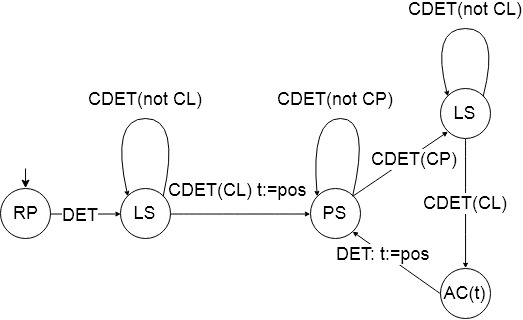
\includegraphics[scale=0.7]{glsm-ils.jpg}
  \caption{General Local Search Machine for ILS}
  \label{fig:ils}
\end{figure}

The simplest acceptance criteria is choice of a better solution, however one may want to use a probabilistic approach. It prevents   major perturbation moves, that do not effectively contribute to objective goal improving, and thus, attains good trade-off between exploration and intensification. History can be taken into account in this heuristics, so the whole procedure is in fact a "Markovian" process, which implies that further moves depend completely on the current state.

\section{Iterated F-Race}

Automatic configuration is a process that optimizes the performance of a certain algorithm as a goal function based on input parameters of the algorithm. The general parameter types are:
 
\begin{itemize}
\item \textbf{categorical} parameters - represent discrete values without any implicit order or distance measure between its possible values. Define the choice of constructive procedure, choice of branching strategies (i. e. algorithmic blocs) and so on.
\item \textbf{ordinal} parameters - are also assigned to finite discrete values, but they have implicit value order (such as \emph{low, middle, high}). Define lower bounds, neighborhoods.
\item \textbf{numerical} parameters - define integer or real values/constants such as weighting factors, population sizes.
\end{itemize}

Some of the parameters maybe subordinate to other ones. This means that their values only make sense if the parameters, that they subordinate to, are assigned to certain values. This can be expressed as a scalar value constraint (e.g $a < b$) or as a dependency on concrete values of some categorical or ordinal parameter. In addition, one can force constraints for several different parameters combined (even the ones of different type).

\begin{figure}
  \centering
    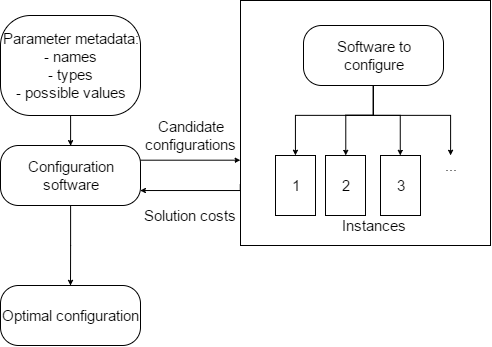
\includegraphics[scale=0.7]{configuration-top-level.png}
  \caption{Automatic configuration scheme}
  \label{fig:autoconf}
\end{figure}

Figure \ref{fig:autoconf} shows the configuration software and software to configure. Configuration script has parameter metadata at its disposal. Based on them, the configuration software runs the software to configure with candidate configurations according to some algorithm. After the configuration process finishes, the configuration software renders the best configurations obtained. In the most general software case there are two measures of the performance - solution quality (to maximize) and computation time (to minimize). This general approach is called an offline tuning. It introduces a learning stage on training instances before learning on the real-world instance set.


A widely used configuration algorithmic family is racing algorithms. The simplified algorithm is shown in Listing \ref{lst:racing} and an illustration is in Figure \ref{fig:irace}.


\begin{minipage}[c, breaklines=true]{0.95\textwidth}
\begin{lstlisting}[caption={General racing pseudo-code}, label={lst:racing}]
procedure racing
start with an initial candidate set Theta
repeat iterations I
	process an instance stream
	evaluate the candidates sequentially
	remove inferior candidates
until winner is selected or exit condition fulfilled
end
\end{lstlisting}
\end{minipage}


\begin{figure}
  \centering
    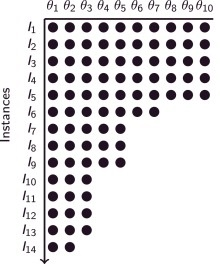
\includegraphics{irace.jpg}
  \caption{irace execution illustration}
  \label{fig:irace}
\end{figure}


Irace (iterated race) configuration implementation was developed and described in \cite{LopDubStuBir2011:techreport-004}. It was implemented in R with taking into account the parallel programming techniques and an initial candidate set-up. It is implemented as an offline tuning. That means, that the tuning is a separate preparatory process from the actual real-world problem application. The feature of the irace is based on iterated generation of new configurations and removing of solutions with lower quality for further evaluating on the problem instances.

In order to tune the configurations that are sampled, irace algorithms uses independent sampling distributions for each of the parameters. For numeric values those are normal distributions and discretely-defined distributions for the rest. The configuration biasing procedure is based on modifying the sampling distributions.

Iterated racing is an automatic configuration implementation that consists of three steps:

\begin{itemize}
\item Sampling new configurations according to a particular distribution.
\item Selecting the best configurations from the newly sampled ones by means of racing.
\item Updating the sampling distribution in order to bias the sampling towards the best configurations.
\end{itemize}

After new configurations are sampled comes the selection stage. At the configuration selection stage, irace runs each of the configurations on a single problem instance from the predefined instance set. After each racing iteration the worst configurations are discarded. Then the rest of the configurations update parameter sampling distributions. The racing stops when the number of the survived configurations becomes small enough (defined by termination criteria).

Some irace extensions can be applied. \textbf{Initial configurations} can be set before the run of the irace. \textbf{Soft-restart} is used for preventing premature convergence. Such convergence may suppresses configuration diversity and, therefore some good configurations may be lost. This restart is triggered if the value of an ad hoc function of configuration distance is lower than a certain margin. Then reinitialization is applied to the elite configurations.


\chapter{Vehicle Routing Problem}


\section{Problem definition}

All variations of the Vehicle Routing Problem (VRP) represent a problem of distribution of goods among the given customers by means of a vehicle fleet. Each edge between nodes is attributed a measure of cost, that represents the distance between these nodes or the time required to travel from one to another. Each customer is attributed its demand of goods. As a goal one usually uses the total distance traveled. However, in some variants the objective can be as follows:

\begin{itemize}
\item Minimize the number of the required vehicles.
\item Minimize variation in travel distances and required capacities, i.e. vehicle fairness.
\item Minimize penalties for low quality service.
\end{itemize}

One may also take into account several objectives at once, thus having a multi-objective optimization problem.

As a basis for the VRP formulation we use the Capacitated Vehicle Routing Problem (CVRP) \cite{CORDEAU2007367}. However minor generalizations are actually implemented in the framework above the given formulation. \par

The CVRP is defined on a complete undirected graph $G=(V,E)$. A set of nodes $V=\{0,1,...,n\}$ is a union of all customer nodes $V\setminus\{0\}$ and a depot node $\{0\}$. Distance $c_e$ or $c_{ij}$ is assigned to each edge $e \in E = \{(i,j): i,j \in V, i<j\}$. The vehicle fleet is represented by $m$ identical vehicles, having a capacity $Q$ and a total distance limit $L$.

The constraints are defined as follows:
\begin{enumerate}
\item Each customer is only visited by exactly one vehicle.
\item Each route starts and ends at the depot.
\item The total demand that any vehicle covers does not exceed the vehicle's capacity $Q$.
\item The total distance that any vehicle passes on route does not exceed the limit L. 
\end{enumerate}

However in addition to this definition one can apply several soothing generalizations:

\begin{enumerate}
\item A \textbf{Non-symmetric matrix} can be considered, i.e. moving an edge one-way may have a different cost from moving the other direction.
\item A \textbf{Non-homogeneous vehicle fleet}. Every vehicle has its own maximum capacity and maximum distance.
\item The \textbf{vehicle may lack of maximum distance restriction}. In other words, the maximum distance can be set to infinity.
\item \textbf{Open/closed problem variations}. The open VRP is a VRP variation, where a vehicle does not have to return to the depot. Closed is a variation, where it must return to the depot in any case. The generalization can be done at the matrix definition step by setting all edges leaving from a customer to the depot to 0 in case of the open VRP. On the contrary, in the closed VRP they are set to their actual travel cost.
\end{enumerate}

Two general feasibility constraints can be verified in advance before solving a problem instance. Firstly, one can check whether the total demand of all customers is not larger than the total supply of all vehicles in the case of rhe limited fleet. Secondly, one can check that the maximum demand of a single customer does not exceed the maximum supply of a vehicle fleet, since only one vehicle supply a customer in the basic VRP model.

A problem is the Traveling Salesman Problem (TSP). TSP is a particular case of closed CVRP, where a single vehicle is used instead of a whole fleet, and all capacity and length constraints are always satisfied. Both of these problems require vehicles to return to the initial node in the general variation. Both problems have an objective defined as the total distance traveled by a vehicle/vehicles. Another way to look at the VRP problem is to consider it a combination of a partitioning problem and routing problem. Partition part defines which elements (customers) are together in one partition (tour). Routing problem  finds the shortest route for the given subset of customers, which corresponds to the TSP problem.

The purpose of the ants is to obtain initial routes, that are biased by the pheromone trail values. The next part of the solution is to improve the obtained routes by means of local search.

In case of limited non-homogeneous vehicle fleet, the results strongly depend on the order of vehicle departure. We propose to emit vehicles in order of their decreasing capacities. By this we try to the maximize number of customers visited by a single vehicle and remove redundant long-distance travels over zones, where customers were already satisfied.

\section{Applying ACO to the VRP}

Applications of ACO algorithms for the VRP are described in various papers. An improved Ant System algorithm for the VRP was introduced by Bullnheimer in \cite{DBLP:journals/anor/BullnheimerHS99}. It uses heuristic information, candidate list and local search. An algorithm called SavingsAnts was described by Doerner in \cite{10.1007/3-540-46004-7_2}. It uses a notion of savings of combining two customers on one tour as opposed to serving them on two different tours. An Ant Colony System algorithm was applied for a dynamic VRP by Montemanni and Gambradella in \cite{MontemanniR.2005ACSf}. ACO metaheuristics may include many various algorithmic options such as using of candidate lists, heuristic values, local search algorithms, solution destruction/reconstruction procedures.

A \textbf{candidate list} can severely boost performance. Similarly to the TSP, a \textbf{cl nearest neighbors} candidate lists can be used. For sake of optimization, these lists are computed once in the beginning of the metaheuristics execution and exploited during the whole run. Such a candidate list must be determined separately for every node.

During the preselection phase, the algorithm will examine the candidate list for the current node in the first place. If none of these will satisfy the constraints (capacity, distance, already visited constraints), only then the nodes outside the candidate list will be considered.

In the VRP and TSP, one typically uses the inverted value of the distance between two nodes as the \textbf{heuristics value}, see \eqref{eq:vrp_heuristic_value}. Thus, the selection phase will bias the tour edge towards shorter ones.

\begin{equation}
\label{eq:vrp_heuristic_value}
\eta_{edge} = 1 / c_{edge}
\end{equation}

Two \textbf{local search} variations are proposed - Or-opt move \cite{Stattenberger2007} and an Iterated Local Search, that uses the underlying Or-opt move, see Listing \ref{lst:ils}.

Illustrations of Or-opt moves are shown in Figures \ref{fig:twohalf}, \ref{fig:twohalf1}, \ref{fig:twohalf2}, \ref{fig:twohalf3}. In an Or-opt move, a replaceable edge $(y1;y2)$ is chosen, and swapped with another sequence of edges, consisting from one up to three customers, denoted by $(x2)$, $(x2,x3)$ or $(x2,x3,x4)$ on the illustrations. Therefore, the size of solution neighborhood is a function depending on tour size of complexity $O(n^2)$.

The whole local search procedure consists of sequential attempts of such local moves by trying all possible position combinations of the replacable edge and the replacing ones. The length of the replacing sequence is defined by a random number generator. In our implementation the local move is applied if it reduces the value of the objective function. However, if a local move was applied, one does not reset the position combinations of the loop, but continue with the current progress. In case if a solution consists of several tours, this procedure is applied to every one of them.

In order to accelerate the computation of the objective function value one may simply subtract the distance of the edges that are removed and add the distances of the edges that are added. Thus, we avoid full tour recomputation. If during the exploration of the neighborhood one applied the local move at least one time, the whole attempt cycle is repeated. Otherwise, it means that we have converged to a local optimum and we keep the current solution. The 2.5-opt pseudo-code is shown in Listing \ref{lst:vrp-two-half}.

\begin{multicols}{2}
\begin{figure*}[ht!]
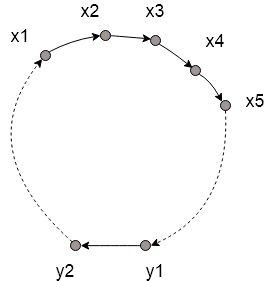
\includegraphics[width=.3\textwidth]{two-half/two-half.jpg}\hfill
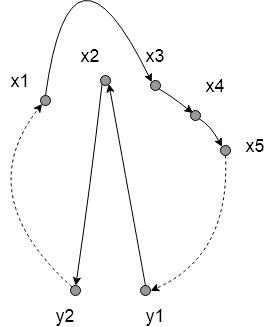
\includegraphics[width=.3\textwidth]{two-half/two-half-1.jpg}\hfill

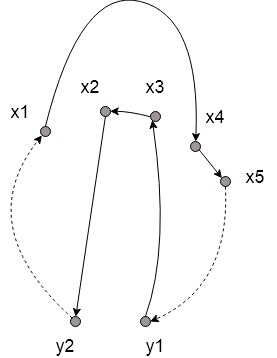
\includegraphics[width=.3\textwidth]{two-half/two-half-2.jpg}\hfill
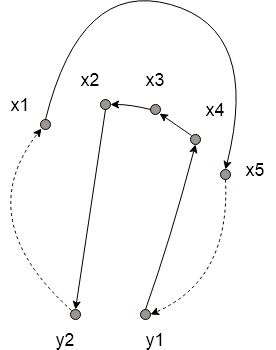
\includegraphics[width=.3\textwidth]{two-half/two-half-3.jpg}
\caption{Initial tour} \label{fig:twohalf}
\caption{Result of swapping with 1 node} \label{fig:twohalf1}
\caption{Result of swapping with 2 nodes} \label{fig:twohalf2}
\caption{Result of swapping with 3 nodes} \label{fig:twohalf3}
\end{figure*}
\end{multicols}

\begin{minipage}[c, breaklines=true]{0.95\textwidth}
\begin{lstlisting}[caption={2.5-opt pseudo-code for VRP problems}, label={lst:vrp-two-half}]
procedure vrp-two-half(solution)

do
  improved = false
  
  for every possible sequence position
    for every possible non-violating exchange node position
      pick random length for sequence from 1 to 3
    
      if this move will reduce the cost
        execute the move
        improved = true
    end
  end
while (improved = true)

end
\end{lstlisting}
\end{minipage}

In addition one may use 2-opt moves that are based on selecting two random non-adjacent edges, swapping two customers between these two edges and reversing the sequence of customers between them. Whether such a move is profitable can also be computed in optimized way.

For ILS in case of VRP problems, one can implement perturbation as double-bridge move, see Figure \ref{fig:dbridge1} and \ref{fig:dbridge2}.

\begin{minipage}[c, breaklines=true]{0.95\textwidth}
\begin{lstlisting}[caption={Iterated Local Search outline}, label={lst:ils},mathescape]
procedure ils(solution s)
	$s_0$ = GenerateInitialSolution
	$s^*$ = LocalSearch($s_0$)
	repeat
		$s'$ = Perturbation($s^*$,history)
		$s^*$' = LocalSearch($s'$)
		$s^*$' = AcceptanceCriterion($s^*$, $s^*$', history)
	until (termination condition met)
end
\end{lstlisting}
\end{minipage}


\begin{multicols}{2}
\begin{figure*}[ht!]
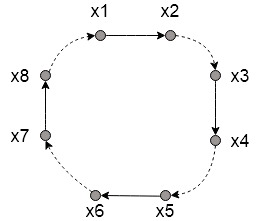
\includegraphics[width=.3\textwidth]{double-bridge/1.jpg}\hfill
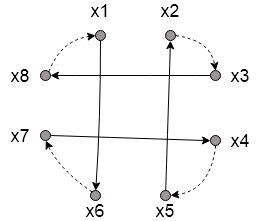
\includegraphics[width=.3\textwidth]{double-bridge/2.jpg}
\caption{Tour before perturbation} \label{fig:dbridge1}
\caption{Tour after applying double-bridge perturbation} \label{fig:dbridge2}
\end{figure*}
\end{multicols}


\textbf{Solution destruction} is a procedure, that is necessary to implement for iterated greedy extensions. A whole range of diverse algorithms can be proposed here only being limited by fantasy. This procedure is necessary to implement for performing iterated ants and cunning ants algorithms. We implemented it as the following stochastic procedure: every tour of a certain solution with certain probability is a subject to slicing. Slicing means that a random number of solution components are removed. At the same moment, the corresponding quantity of length-capacity and supply-capacity is updated to the vehicle of the sliced tour, so refinishing of the tour can be done. The objective function is also updated to the one of the obtained partial solution. Still, the initial "parent" objective function value has to be backed-up, in order to be able to compare partially destroyed solutions in External memory during tournament selection process.

In our implementation the solution is reconstructed in the same way as in the normal construction. This means that an ant continues the tour from the last customer visited and visits the rest of the nodes, being biased by pheromone trail values and problem constraints.



\chapter{Implementation}


\section{Software design}

The software framework is implemented in Java 1.8.0 in correspondence with the object-oriented programming paradigm. Besides VRP, many other combinatorial optimization problems are also anticipated to be solved by means of this framework. This framework remains highly flexible and adaptive in terms of problem variations. This is attained by design patterns and deep abstraction of the framework components. Consistent application of abstractions ensures minor code-repetition, being ready for some algorithm modifications. The dependency injection concept ensures, that the high-level abstractions do not determine the low-level details themselves. Instead, they only receive these dependencies as arguments. This also allows to resort to white-box unit testing of some software components.

All classes are strictly grouped in two parts. The first part comprises the \textbf{problem independent} classes. The second part comprises the problem dependent classes. Problem independents are:

\begin{itemize}
\item \textbf{Solver}, which is an abstract class that encapsulates high-level metaheuristics, that aim to solve abstract combinatorial optimization problems. It is the central class in the framework. It also contains all shared lower-level algorithmic components, such as problem instance itself, solution component selector, termination criteria, local search, pheromone initializer, local and global update strategies. Basic abstract operations are already implemented in this class such as constructing one abstract solution of an abstract problem. Abstract solution description will be given later.

\item \textbf{SolverStandard} - ACO algorithm without any iterated greedy or other extensions.

\item \textbf{SolverIteratedAnts} - ACO algorithm with iterated ants as iterated greedy extension. Also holds an IteratedCriteria.

\item \textbf{IteratedCriteria} - an algorithm that gives preference to either one solution or another. It is used in SolverIteratedAnts. Can be either deterministic or probabilistic.

\item \textbf{SolverExternalMemory} - ACO algorithm with iterated ants as iterated greedy extension. Also contains TournamentSelector.

\item \textbf{TournamentSelector} - a procedure used in SolverExternalMemory, that selects certain number of solutions from a given set according to the tournament selection rule.

\item \textbf{SolverCunningAnts} - ACO algorithm with cunning ants as iterated greedy extension. Is is also obliged to use MMAS as global update strategy.

\item \textbf{Problem} - is an encapsulation of an abstract problem. It contains general problem components such as CandidateDeterminer, ComponentStructure and a flag whether it is a maximization or minimization problem.

\item \textbf{Component} - encapsulates an abstract problem solution component. Allows computation of its selection weight. Performs caching of the selection weight, so it gets rid of redundant recomputations.

\item \textbf{ComponentStructure} - contains the solution components in an unspecified data structure (matrix in case of VRP).

\item \textbf{CandidateDeterminer} - generates an abstract, problem-specific CandidateList.

\item \textbf{CandidateList} - abstract, problem-specific candidate list. It is computed once before the run.

\item \textbf{Solution} - encapsulates an abstract, problem-independent solution of an abstract problem. It must have an objective function value, that is updated during the construction run according to the problem formulation. It also must have a procedure of obtaining a solution component set that is available at the current construction step. Also deep copying method must be implemented, since it is widely used by solvers and local search strategies. Deep copying implies that all comprised objects (arrays, lists, solution tours) are copied too, not simply leaving the reference copies.

\item \textbf{GlobalUpdate} - abstract global pheromone update strategy. It includes a standard evaporation method, since it is shared by most of the global updates.

\item \textbf{AntSystem}, \textbf{AntColonySystem}, \textbf{MinMaxAntSystem}, \textbf{RankBasedAntSystem}, \textbf{ElitistAntSystem}, \textbf{BestWorthAntSystem} - correspond to the respective global update strategies. MMAS in addition contains PheromoneTrailSmoothing.

\item \textbf{PheromoneTrailSmoothing} - is used bu MMAS. As an optional step.

\item \textbf{LocalUpdate} - optional argument in the general case and mandatory in case of choosing AntColonySystem as a global update strategy.

\item \textbf{LocalSearch} - high-level hybrid SLS. May use Move class as low-level components.

\item \textbf{IteratedLocalSearch} - performs an iterated local search. Depends on Perturbation and Move strategy. High level class, that is not dependent on a problem type.

\item \textbf{Move} - simple SLS. It performs local move, that is used by hybrid SLS.

\item \textbf{Selector} - an abstract stochastic algorithm that selects a solution component out of a set of components according to some stochastic rule, by taking into consideration the pheromone trail and heuristic values of these components.

\item \textbf{TerminationCriteria} - abstract solver termination criterion. Implemented as time criteria and number of iterations criteria for unit testing.

\item \textbf{PheromoneInitializer} - an abstract strategy that initializes/reinitializes pheromone trail values for a whole ComponentStructure. Normally implemented as a stochastic operation.

\end{itemize}

A feature of problem-dependent is that they may be easily substituted by others, thus switching the framework application. It is only necessary to implement certain low-level methods for them, such as implementing of possible solution components, problem-specific local searches and solution destroyers, determining solution component candidate lists , etc. Those are:

\begin{itemize}
\item \textbf{Problem2d} - extends Problem class. Encapsulates a problem, that has a two-dimensional matrix organization of its solution components.

\item \textbf{ProblemVRP} - encapsulates a VRP problem instance.

\item \textbf{ComponentStructure2d} - a ComponentStructure implementation for Problem2d. Implemented as dense matrix of solution components and sparse matrix of solution components by means of a hash table. The latter allows to have some memory consumption gain, however it cannot be used specifically for the VRP problem, due its dense definition of solution components.

\item \textbf{ParserVRP} - VRP problem instance parsing. May have many implementations, since one problem type may have many formats of representation.

\item \textbf{Vehicle} - encapsulation of a vehicle. Contains information related to capacity and distance constraints.

\item \textbf{Fleet} - abstract class, that contains a sequence of vehicles. Generates a vehicle iterator for their sequential emission during solution process. The order of emission depends on a particular implementation of this class.

\item \textbf{Tour} - is an inherent part of the VRP problem solution. A set of tours defines a solution. One tour is associated with one predefined vehicle. It contains the current consumption of capacity and distance, remaining capacity and distance, list of visited nodes, associated vehicle pointer.

\item \textbf{SolutionVRP} - is a solution of a VRP problem instance. It contains all selected solution components, array of flags of visited customers with, vehicle iterator (generated by Fleet class), all solution tours, and current solution construction progress information.

\end{itemize}



Design patterns are widely used during the development process. One of the most used patterns here are "Strategy", "Command" and "Template method", due to having a varied range of algorithms on different levels, that adhere to some common structure. All concrete implementation in the program entry point are inferred from the program arguments and are created by means of many "Factory methods" in the \textbf{Launcher} class. "Prototype" pattern is used for \textbf{Solution} class and its sub-classes in order to be able to clone solutions one from another as it is required by some algorithms. "Iterator" is used for the vehicle fleet for obtaining a sequence of vehicles, that build a solution in order of their emission.



\section{Preselection stage}

Generally, in ACO algorithms there are two ways of maintaining feasibility of solutions. The first is two ensure solution \textbf{feasibility at every moment} of the run, the second is to \textbf{allow processing unfeasible solutions}, however trying to bias towards the solution components, that keep or likely keep the solution feasible. The second possibility is good for solving problems with complicated constraints that require a lot of computations in order to keep or make them feasible. In the VRP, however, we have decided to use the first approach. This will allow to avoid unnecessary construction of solutions, that are expected to be unfeasible beforehand. \par

Before applying selectors according to formulas \eqref{eq:construction_classic}, \eqref{eq:construction_maniezzo} or \eqref{eq:construction_dorigo} (see Page \pageref{eq:construction_classic}) one has to determine the possible solution components at the current construction step. The proposed preselection algorithm is shown in Listing \ref{lst:preselection}. It selects all edges that do not violate any constraint. Among such constraints there are non-revisiting, not going to itself, not going to the depot edges. Out of those several are filtered out, such as the ones, that violate the capacity constraint and distance constraint. In particular, we ensure condition $leftDistance >= dist(current;N) + dist(N;depot)$, since it does not make sense to go by a certain edge, if it will not be possible even to return to the depot from it. Neither it will be possible to return to the depot by going any farther from that node, which is ensured by triangle inequality property, that works in all VRP instances, which are based on Euclidean space. In case if no such node is found, then the vehicle returns directly to the depot from the current node.

In case if a candidate list is used, then the initial set is populated from this list, and the constraints are applied after.

\begin{minipage}[c, breaklines=true]{0.95\textwidth}
\begin{lstlisting}[caption={Solution component preselection pseudo-code}, label={lst:preselection}]
procedure preselection(currentNode)
	foreach non-visited non-loop non-depot-leading node N
		if leftCapacity >= demand(N)
			if leftDistance >= dist(current;N) + dist(N;depot)
				add component(current;N) to resultSet
			end
		end
	end
	
	if size(resultSet) == 0
		add component (current;depot) to result set
	end
		
	return resultSet
end
\end{lstlisting}
\end{minipage}


\section{Configuration process set-up}

By aggregating all options, strategy choices and flags, one forms a parameter space according to Table \ref{tbl:space} on Page \pageref{tbl:space}. This parameter space formulation corresponds to the irace representation. Every parameter is defined by its i-race name, publicly known alias (or new if such was not invented), type, possible parameter values, condition of validity. Every parameter can be categorical, integer or real. In case of integer and real parameters lower and upper bounds of the possible values are specified. In case of categorical all possible values are listed. Condition is a predicate, that defines whether this parameter must be assigned a value, or this parameter must not present in the generated configuration.


In addition to the conditional restrictions, several additional constraints have to be ensured by means of forbidden configuration file.

\begin{itemize}
\item Ant Colony System only works with standard or Dorigo selectors.

\item Ant Colony System must use local update.

\item In external memory $topK$ has to be equal or less than the ant number $m$.

\item Cunning ants must use MMAS as global update technique.
\end{itemize}


\section{Testing}


All parameter constraints are checked on two levels. Firstly, the irace scenario is set in such a way, that it will only generate valid configurations by means of conditional parameters and specification of forbidden configurations. Secondly, configuration is wholly scanned in the framework itself, not only by checking valid parameter bounds, but also by verifying consistency between several parameters. In case of inconsistency, the framework returns a verbal exception response with error description.

Thorough unit and integrated testing is done in order to validate the performance of the framework. Several auxiliary problem instances are used in order to simulate very specific artificial situations. Both white-box and black-box methodologies are used depending on a test case. For white-box mock objects are used to test specific method calls/returns by tested objects. This is done by using the Mockito framework in combination with JUnit library. Random seed forcing is used to switch execution behavior
from pseudo-random to deterministic, thus ensuring a concrete scenario.

\chapter{Experimental}

While running the framework on certain instances one must remember, that performance of a run is a cumulative result of several factors at a time: 

\begin{itemize}
\item Performance of a concrete configuration.
\item Features of a concrete problem instance.
\item Performance of hardware and run conditions.
\item Run-time.
\end{itemize}

To make configuration benchmark more fair, all factors except the configuration itself must be equalized. The runs must be done on same hardware in same or at least roughly same run conditions. Majorana computation cluster was used for this experiments. The precise configuration is given below.
\begin{itemize}
\item 32 computational nodes
\item 2 INTEL Xeon E5410 (4 cores each, 2.33GHz, 2x 6MB L2 cache)
\item RAM per job:450MB
\end{itemize}

The runtime is set as a value, depending on size of an instance: $runtime = num_{nodes} / 2$ (in seconds).

In addition, one must also take into account that, although deterministic behavior of the program can assured by forcing a random seed, one can not guarantee the same result of the program run even with the same configuration, since number of iterations, that will be effectively done within the specified time range, may vary.

\section{Train and test runs}

In order to be able to perform benchmark comparison of the framework's performance, one may use publicly known instances of CVRP problems, see Appendix. To make the performance estimation more objective, one must strictly separate training (tuning) and testing set. This will remove the possibility of that, the results obtained are biased by overfitting, made by the tuning process on concrete instances. For the training stage all Uchoa et al.(2014) instances were selected, that were of size less than 300. These instances are generated on a square grid in Euclidean space. For test instances Golden et Al. (1998) were chosen.

In the end of 20 iterations/20 configurations irace tuning, a presumably good configuration was found. Then, runs of this configuration on test instances were made. The Solution Quality Distribution is shown on Figure \ref{fig:sqd-golden}.

\begin{figure}[h]
  \centering
    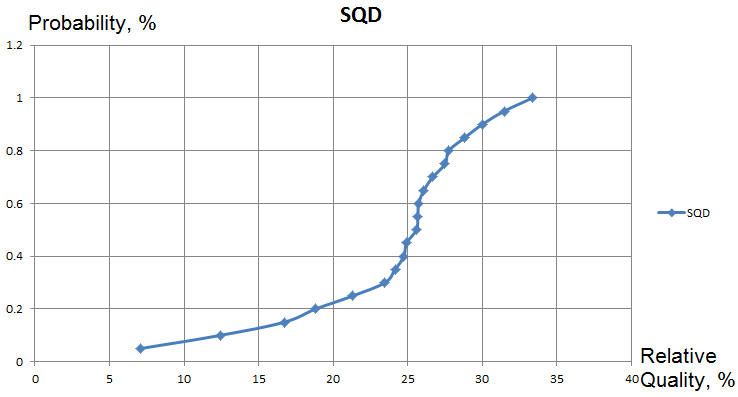
\includegraphics[scale=0.8]{sqd-golden.png}
  \caption{Solution Quality Distribution over Golden et. Al instances}
  \label{fig:sqd-golden}
\end{figure}

The configuration is shown in Table \ref{tbl:obtained}.

In that configuration Dorigo selector is chosen, which may be explained by good balance between exploration and exploitation. The heuristics information impact strongly dominates over the pheromone trail value impact. This however will work only if heuristics information is computed duly, as in our case (inverse value of edge distance). Candidate lists are not used, probably since high beta values already manage to cut off the most of poorly promising edges. EAS is used as global update technique. Local update is used. Iterated greedy heuristics is iterated ants. 2.5-opt is used as local search algorithm. The elitist ant factor is 90, which is very high. Reinitialization time is $0.13 \times runtime$, which means that reinitialization will be only enacted 7 times during the run. The iterated ants solution choice criteria is strictly best.



\section{Existing configuration verification}

In addition to the best configuration obtained, one could use a publicly discovered configurations in literature, \cite{DBLP:journals/anor/BullnheimerHS99}. One can run the replication of that configuration on the same instances (Christofides, Mingozzi and Toth 1979). The SQD of the Bullnheimer and its replication are shown on Figure \ref{fig:sqd-bullheimer-obtained}.

\begin{figure}[h]
  \centering
    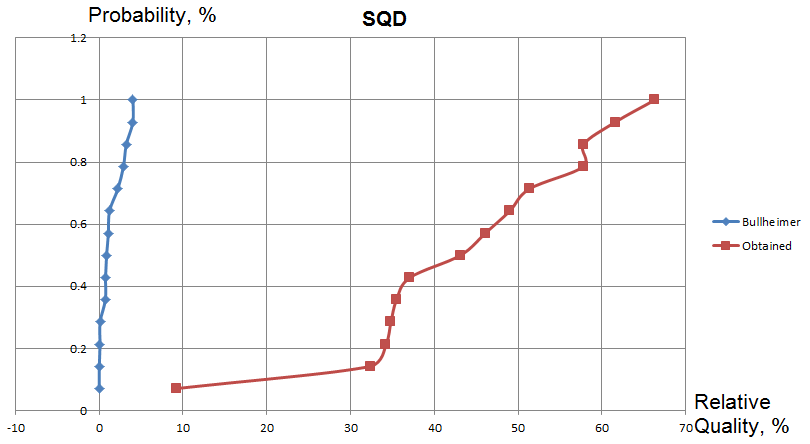
\includegraphics[scale=0.8]{sqd-bullnheimer-obtained.PNG}
  \caption{Solution Quality Distribution for Bullnheimer and its replication}
  \label{fig:sqd-bullheimer-obtained}
\end{figure}

The replication did not show as good results as the original, which might be explained by lesser runtime performed or by differences in some implementation details.




\chapter{Conclusion}

As we were planning, we carried out analysis of the state-of-the-art variations and components of the Ant Colony Optimization algorithms. We managed to emphasize the common traits of those algorithms and designed an object-oriented framework, encompassing thereof. This framework was later implemented in Java. This will allow to run and extend this framework in a platform independent way.

To apply the framework to actual problems, the framework was adapted for Vehicle Routing Problems, which belongs to NP-hard problems.

Then we integrated this framework with a configuration tuning software called irace, created a tuning script and framework parameter specification. The tuning process was performed on Majorana computation cluster.

We performed training (tuning) and testing of the framework on two different publicly known instance sets. In addition, we tried to replicate a publicly known configuration in order to perform benchmark comparison.

This framework in combination with the irace tuning can be used for every combinatorial optimization problem by applying any custom developed ACO metaheuristics. In context of VRP problem, it can be used for transport logistics, microchip design, computer network planning, agriculture, job scheduling, X-Ray crystallography.



\appendix

\backmatter

\printindex % use makeindex to generate the index



\bibliographystyle{plain}

\bibliography{biblio} %use bibtex to generate the bibliography

% BIBLIOGRAPHY DOES NOT WORK IN TEXMAKER, USE OVERLEAF FOR FINAL GENERATION

\chapter{Appendix}

The framework sources, automatic configuration setup, problem instances, analysis results and documentation are available on \url{https://github.com/ElderMayday/master}.

Public CVRP problem instances are available on \url{http://vrp.atd-lab.inf.puc-rio.br/index.php/en/}.

Mockito Testing framework is available on \url{http://site.mockito.org/}.


\begin{table}[]
\centering
\caption{Parameter space for the framework in context of VRP}
\label{tbl:space}
\begin{tabular}{|c|c|c|p{4cm}|p{4cm}|}
\hline
\textbf{Name}  & \textbf{Alias}      & \textbf{Type} & \textbf{Possible values}                                                                & \textbf{Condition}                                                                                     \\ \hline
selector                        & -          & c    & (selector-standard, selector-dorigo, selector-maniezzo)                          & -                                                                                             \\ \hline
alpha                           & $\alpha$   & r    & (0.1,5.0)                                                                      & selector in c("selector-standard", "selector-dorigo")                                          \\ \hline
beta                            & $\beta$    & r    & (0.1,5.0)                                                                      & selector in c("selector-standard", "selector-dorigo")                                          \\ \hline
alpha\_maniezzo                 & $\alpha$   & r    & (0.0,1.0)                                                                      & selector == "selector-maniezzo"                                                               \\ \hline
dorigo\_probability             & $q_0$      & r    & (0.0,1.0)                                                                      & selector == "selector-dorigo"                                                                 \\ \hline
candidate\_list                 & -          & c    & (candidate-yes, candidate-no)                                                   & -                                                                                             \\ \hline
candidate\_ratio                & $r_{cand}$ & r    & (0.0,1.0)                                                                      & candidate\_list == "candidate-yes"                                                            \\ \hline
global\_update                  & -          & c    & (ant-s, ant-colony-s, min-max-s, rank-based-ant-s, elitist-ant-s, best-worst-ant-s) & -                                                                                             \\ \hline
local\_update                   & -          & c    & (local-update-yes, local-update-no)                                             & selector in c("selector-standard", "selector-dorigo")                                          \\ \hline
iterated\_greedy                & -          & c    & (standard, external-memory, iterated-ants, cunning-ants)                          & -                                                                                             \\ \hline
ant\_num                        & m          & i    & (1,50)                                                                         & -                                                                                             \\ \hline
lupd\_epsilon                   & $\epsilon$ & r    & (0.0,1.0)                                                                      & local\_update == "local-update-yes"                                                           \\ \hline
lupd\_tau0                      & $\tau_0$   & r    & (0.0,1.0)                                                                      & local\_update == "local-update-yes"                                                           \\ \hline
local\_search                   & -          & c    & (local-search-none, local-search-ils-twohalf, local-search-twohalf)              & -                                                                                             \\ \hline
ils\_iterations                 & $iter_{ils}$ & i    & (1,30)                                                                         & local\_search == "local-search-ils-twohalf"                                                   \\ \hline
evaporation\_remains            & $1-\rho$   & r    & (0.2,1.0)                                                                      & -                                                                                             \\ \hline
ant\_s\_is\_bounded             & -          & c    & (ant-s-bounded-yes, ant-s-bounded-no)                                           & global\_update == "ant-s"                                                                     \\ \hline
\end{tabular}
\end{table}


\begin{table}[]
\centering
\begin{tabular}{|c|c|c|p{4cm}|p{4cm}|}
\hline
\textbf{Name}  & \textbf{Alias}      & \textbf{Type} & \textbf{Possible values}                                                                & \textbf{Condition}                                                                                     \\ \hline
ant\_s\_k                       & $k$        & r    & (1.0,10.0)                                                                     & (global\_update == "ant-s") \& (ant\_s\_is\_bounded == "ant-s-bounded-yes")                   \\ \hline
min\_max\_s\_p\_best            & $p_{best}$ & r    & (0.01,1.0)                                                                     & global\_update == "min-max-s"                                                                 \\ \hline
min\_max\_s\_global\_best       & -          & c    & (min-max-s-global-best-yes, min-max-s-global-best-no)                           & global\_update == "min-max-s"                                                                 \\ \hline
min\_max\_s\_global\_iterations & $iter_{mg}$ & i    & (1,30)                                                                         & (global\_update == "min-max-s") \& (min\_max\_s\_global\_best == "min-max-s-global-best-yes") \\ \hline
min\_max\_s\_pts                & -          & c    & (min-max-s-pts-yes, min-max-s-pts-no)                                           & global\_update == "min-max-s"                                                                 \\ \hline
min\_max\_s\_pts\_iterations    & $iter_{pts}$ & i    & (1,30)                                                                         & (global\_update == "min-max-s") \& (min\_max\_s\_pts == "min-max-s-pts-yes")                  \\ \hline
pts\_lambda                     & $\lambda$  & r    & (0.0,1.0)                                                                      & (global\_update == "min-max-s") \& (min\_max\_s\_pts == "min-max-s-pts-yes")                  \\ \hline
pts\_ratio                      & $\Omega'$  & r    & (0.0,1.0)                                                                      & (global\_update == "min-max-s") \& (min\_max\_s\_pts == "min-max-s-pts-yes")                  \\ \hline
pts\_delta                      & $\delta$   & r    & (0.0,1.0)                                                                      & (global\_update == "min-max-s") \& (min\_max\_s\_pts == "min-max-s-pts-yes")                  \\ \hline
ras\_w                          & $w$        & i    & (1,30)                                                                         & global\_update == "rank-based-ant-s"                                                          \\ \hline
ras\_is\_bounded                & -          & c    & (ras-bounded-yes, ras-bounded-no)                                               & global\_update == "rank-based-ant-s"                                                          \\ \hline
eas\_m\_elite                   & $m_{elite}$ & i   & (1, 100)                                                                       & global\_update == "elitist-ant-s"                                                             \\ \hline
eas\_is\_bounded                & -          & c    & (eas-bounded-yes, eas-bounded-no)                                               & global\_update == "elitist-ant-s"                                                             \\ \hline
bwas\_mutation\_probability     & $p_{mut}$    & r    & (0.0,1.0)                                                                      & global\_update == "best-worst-ant-s"                                                          \\ \hline
reinitialization                & -          & c    & (reinitialization-yes, reinitialization-no)                                     & -                                                                                             \\ \hline
reinitialization\_time          & $t_{reinit}$ & i    & (0.01,0.2)                                                                     & reinitialization == "reinitialization-yes"                                                    \\ \hline
\end{tabular}
\end{table}


\begin{table}[]
\centering
\begin{tabular}{|c|c|c|p{4cm}|p{4cm}|}
\hline
\textbf{Name}  & \textbf{Alias}      & \textbf{Type} & \textbf{Possible values}                                                                & \textbf{Condition}                                                                                     \\ \hline
top\_k                          & $topK$     & i    & (1,5)                                                                          & iterated\_greedy == "external-memory"                                                         \\ \hline
memory\_size                    & $mem$      & i    & (10,30)                                                                        & iterated\_greedy == "external-memory"                                                         \\ \hline
tournament\_selector\_size      & $tSize$    & i    & (2,10)                                                                         & iterated\_greedy == "external-memory"                                                         \\ \hline
criteria                        & -          & c    & (iterated-criteria-best, iterated-criteria-probabilistic)                       & iterated\_greedy	== "iterated-ants"                                                           \\ \hline
probabilistic\_best             & $p_{iter}$ & r    & (0.0,1.0)                                                                      & (iterated\_greedy == "iterated-ants") \& (criteria == "iterated-criteria-probabilistic")       \\ \hline
destruction\_probability        & $p_{destr}$  &  r & (0.0,1.0)                                                                      & iterated\_greedy in c("external-memory", "iterated-ants", "cunning-ants")                     \\ \hline
\end{tabular}
\end{table}



\begin{table}[]
\centering
\caption{List of parameters of the best configuration obtained}
\label{tbl:obtained}
\begin{tabular}{|l|l|}
\hline
\textbf{Parameter}       & \textbf{Value}         \\ \hline
selector                 & selector-dorigo        \\ \hline
alpha                    & 0.2                    \\ \hline
beta                     & 3.56                   \\ \hline
dorigo\_probability      & 0.72                   \\ \hline
candidate\_list          & candidate-no           \\ \hline
global\_update           & elitist-ant-s          \\ \hline
local\_update            & local-update-yes       \\ \hline
iterated\_greedy         & iterated-ants          \\ \hline
ant\_num                 & 6                      \\ \hline
lupd\_epsilon            & 0.46                   \\ \hline
lupd\_tau0               & 0.19                   \\ \hline
local\_search            & local-search-twohalf   \\ \hline
evaporation\_remains     & 0.66                   \\ \hline
eas\_m\_elite            & 90                     \\ \hline
eas\_is\_bounded         & eas-bounded-yes        \\ \hline
eas\_k                   & 4.02                   \\ \hline
reinitialization         & reinitialization-yes   \\ \hline
reinitialization\_time   & 0.13                   \\ \hline
criteria                 & iterated-criteria-best \\ \hline
destruction\_probability & 0.15                   \\ \hline
\end{tabular}
\end{table}


\end{document}
